\chapter{Présentation du sujet}
Mon sujet s'inscrit dans un projet developpé en interne, le projet SisellBox. Ansi,
je vais présenter dans un premier temps le projet, puis dans un second temps
expliquer ou je m'inscrit dans le projet et qu'est ce que j'y apporte.



\section{Le projet SisellBox}
\label{sisselbox}

\begin{figure}[!h]
  \centering
  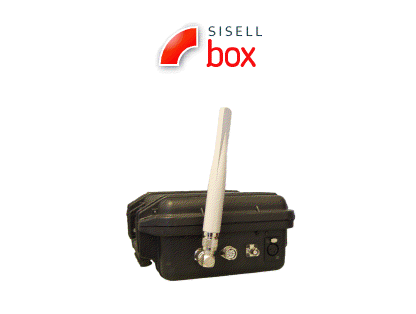
\includegraphics[scale=0.7]{figures/sbox}
  \caption{ci dessus une image de la SisellBox}
\end{figure}
\newpage
La Sisell Box est un enregistreur développé par Open Wide permettant de déployer une solution complète de vidéo surveillance rapidement.
Ce système peut être utilisé dans des contextes de mission très différents : surveillance longue durée, protection de sites sensibles, capture d'images hautes qualité, ainsi que surveillance ponctuelle.
Fonctionnant sur batterie et créant un réseau wifi maillé de façon autonome, elle ne nécessite que peu d'intervention humaine pour l'utilisation. Il suffit de brancher la batterie, brancher les caméras et elle est autonome. L'utilisation d'algorithmes performants lui permet de détecter et d'analyser tout événement (intrusion, stationnarité, mouvement de foule) sur la base de critère précis et configurables. Le projet Sisell se découpe en partie, deux partie, d'une part le "streamer", prenant en entrée une source vidéo "live"(par exemple une caméras de sécurité) et fourni un flux de composé de vidéo et de métadonnées.



\chapter{La problématique posé}
\begin{itemize}
  \item Etude de Gstreamer
  \item Etude du protocole MPEG-TS
  \item Transmission de flux vidéo + métadonnée
  \item patch du plugin Gstreamer mpegtsmux afin de  multipler les donnes
  \item patch du plugin de Gstreamer mpegtsdemux afin demultplexer les données pour le stockage
  \item afficher les metadonnée sur une une interface a
\end{itemize}
